\chapter{Lösungsansatz} \label{chapter2}
\section{Grundlegender Lösungsansatz}
% sortieren nach Zeitraum
Die gegebenen Werte für die Aufgabe sind die Startzeit (8 Uhr) und die Endzeit (18 Uhr) einer Reservierung. Dazu kommt noch die Länge der Reservierung. Grundlegend gewinnt eine Reservierung an Wert, je mehr sie an Zeit einnimmt. Eine Reservierung ist besonders wertvoll, wenn sie von 8 - 18 Uhr geht. Das liegt daran, dass der komplette verfügbare Platz von der Reservierung \texttt{ra} eingenommen wird und keine andere Reservierung \texttt{rn} neben \texttt{ra} passt. Würde \texttt{ra} nur von 8 - 16 Uhr gehen entsteht Fehlerpotential. Folglich werden bessere Lösungen gebildet, wenn die Reservierungen nach der überstrichenen Zeit sortiert werden. Das Sortieren der Reservierungen legt einen guten Grundstein für weitere Optimierungsverfahren. (vgl. Abbildung \ref{fig:bsp:unsortiert} und Abbildung \ref{fig:bsp:sortiert})\par
% Bilder zur Visualisierung
\begin{minipage}{.5\linewidth}
\begin{figure}[H]
    \centering
    
\includegraphics[scale=0.25]{images/unsortiertes_beispiel.png}
    \caption{unsortiertes Beispiel}
    \label{fig:bsp:unsortiert}
\end{figure}
\end{minipage}
\begin{minipage}{.5\linewidth}
\begin{figure}[H]
    \centering
    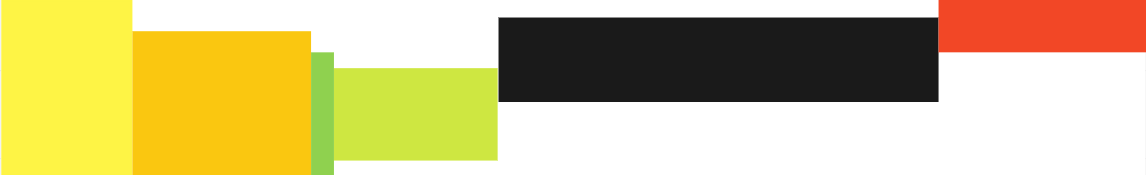
\includegraphics[scale=0.25]{images/sortiertes_beispeil.png}
    \caption{sortiertes Beispiel}
    \label{fig:bsp:sortiert}
\end{figure}
\end{minipage} \par
% einsortieren von Reservierungen
Als nächstes müssen Reservierungen einsortiert werden. Würde man die Reservierungen zu diesem Zeitpunkt sortiert in den \textit{Bin} einschreiben und den Anfang der Reservierung gleich das Ende der vorherigen Reservierung setzten, hält sich das Ergebnis von der Souveränität in grenzen. Um noch ein besseres Ergebnis zu erhalten werden die Reservierungen soweit wie möglich nach links einsortiert. Die Reihenfolge dabei orientiert sich nach der Sortierung. Die erste Reservierung wird bei der X Koordinate \texttt{x\_pos} 0 eingeordnet. Die nachfolgenden Reservierungen werden der nächsten freien Position zugeordnet. Dabei kann es zwei mögliche Szenarien geben. In beiden geht die Reservierung \texttt{ra} von 8 - 16 Uhr und nimmt 300 Meter an Platz ein. Die folgende Reservierung \texttt{rn} geht in dem ersten Szenario von 16 - 18 Uhr und somit überschneiden sich \texttt{ra} und \texttt{rn} von der Zeit nicht. Die \texttt{x\_pos} von \texttt{rn} ist ebenfalls 0. In dem zweiten Szenario geht \texttt{rn} von 14 - 18 Uhr und somit überschneiden sich die Start- und Endzeiten der Reservierungen. Deswegen muss sich \texttt{rn} hinter \texttt{ra} einordnen und bekommt die \texttt{x\_pos} 300 zugewiesen.\par
% ein weiterer Sonderfall
In dem vorher geschilderten Szenarios kann es durchaus passieren, dass die Reservierung \texttt{rn} mit dem Zusammenspiel aus Position und Länge über 1000 geht. Damit wäre die Reservierung invalide und wird von dem Algorithmus in ihrer \texttt{x\_pos} mit -1 versehen. Eine Reservierung mit -1 wird am Ende des Algorithmus ignoriert.

\section{Erweiterter Lösungsansatz}
% Einleitung
Dadurch, dass alle Objekte für jede Position getestet werden müssen leidet die Laufzeit sehr. Deswegen wird nun ein System thematisiert, welches das Gleiche in einer minimalen Laufzeit erledigt.\par
% Vorstellung vom Line-System
Die Iterationen lassen sich begrenzen, indem nur die Reservierungen \texttt{ra} genommen werden, welche mit der Reservierung \texttt{rn} interferieren. Ob \texttt{ra} mit \texttt{rn} interferieren wird mit einem \textit{Tensor} ermittelt. Die X-Achse des \textit{Tensors} ist die Endzeit und die Y-Achse die Startzeit der Reservierung. Nach diesem Prinzip ist es nicht möglich ein Element bei den Indizes \texttt{[0][0]} zu haben, da eine Reservierung nicht um 8 Uhr starten kann und wieder um 8 Uhr aufhören. Die Z-Achse des Tensors sind dann die Elemente. Generell lässt sich der Tensor als Matrix darstellen, da die Z-Achse nur zum speichern dient und so nicht dargestellt werden muss. Die folgende Darstellung \ref{fig:matrix_valide_indizes} zeigt den Tensor als Matrix mit den validen Bereich markiert.
\begin{figure}[H]
    \centering
    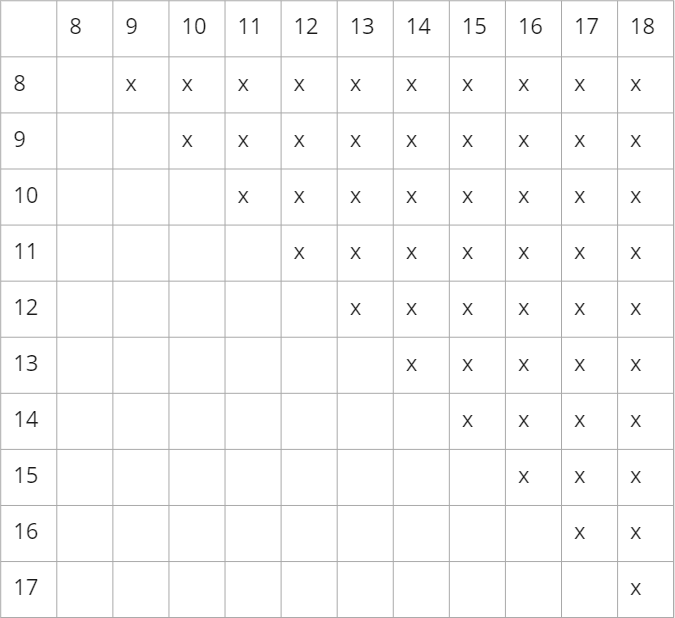
\includegraphics[scale=0.55]{images/matrix_valide_indizes.png}
    \caption{Matrix mit validen Indizes}
    \label{fig:matrix_valide_indizes}
\end{figure} \par
Wenn \texttt{rn} einsortiert werden soll so wird in einem bestimmten Bereich von der Matrix ausgewählt. Der Bereich hängt von der Start- und Endzeit von \texttt{rn} ab. Die Startzeit nimmt Einfluss auf den Index der X-Achse (erste Dimension). Wenn die Startzeit 9 Uhr ist, dann darf eine Reservierung \texttt{ri} aus \texttt{ra} noch um 9 Uhr Enden, aber wenn \texttt{ri} um 10 Uhr endet kollidieren die beiden Reservierungen. Der Bereich geht auf der X-Achse immer bis zum Ende der Matrix, da sobald die Endzeit einen bestimmten Wert überschritten hat, wird \texttt{ri} immer mit \texttt{rn} interferieren. Der Index der zweiten Dimension hängt von der Endzeit der Reservierung \texttt{rn} ab. Endet \texttt{rn} um 16 Uhr können Reservierungen um 16 Uhr anfangen und nicht mit \texttt{rn} kollidieren. Die beiden in diesem Abschnitt aufgestellten Rechnung werden im Abschnitt ???? nochmals genauer thematisiert. \par
